\documentclass[11pt]{article}

\usepackage{amsmath, amssymb, amsthm}
\usepackage{geometry}
\usepackage{hyperref}
\hypersetup{pdfencoding=auto}
\usepackage{booktabs}
\usepackage{graphicx}
\usepackage{microtype}
\usepackage{enumitem}
\usepackage{xcolor}
\usepackage{doi}

\geometry{margin=1in}

\newtheorem{theorem}{Theorem}[section]
\newtheorem{proposition}[theorem]{Proposition}
\newtheorem{lemma}[theorem]{Lemma}
\newtheorem{corollary}[theorem]{Corollary}
\theoremstyle{definition}
\newtheorem{definition}[theorem]{Definition}
\newtheorem{example}[theorem]{Example}
\theoremstyle{remark}
\newtheorem{remark}[theorem]{Remark}
\newtheorem{conjecture}[theorem]{Conjecture}
\newtheorem{hypothesis}[theorem]{Hypothesis}

\DeclareMathOperator{\rank}{rank}
\DeclareMathOperator{\spn}{span}
\DeclareMathOperator{\Cl}{Cl}
\DeclareMathOperator{\PSL}{PSL}
\DeclareMathOperator{\SL}{SL}
\DeclareMathOperator{\tr}{tr}
\DeclareMathOperator{\Id}{Id}
\newcommand{\R}{\mathbb{R}}
\newcommand{\C}{\mathbb{C}}
\newcommand{\F}{\mathbb{F}}
\newcommand{\Hmat}{\mathcal{H}_{\mathrm{mat}}}
\newcommand{\Tmat}{\mathcal{T}_{\mathrm{mat}}}
\newcommand{\peff}{\widetilde{p}}
\newcommand{\rbmat}{\tilde{r}^{B,\mathrm{mat}}}
\newcommand{\deff}{|\partial^{B,\mathrm{mat}} S_n|}
\newcommand{\beff}{\beta_{\mathrm{eff}}}
\newcommand{\Rn}{\mathcal{R}_n}

\title{Matrix-Level Dynamic Redundancy and the Structural Confinement\\
of the Cascade Exponent $\beta$}

\author{J\'{e}r\^{o}me Beau\\
\small Independent Researcher; jerome.beau@cosmochrony.org}

\date{March 2026}

\begin{document}

  \maketitle

  \begin{abstract}
    The Cosmochrony spectral relaxation programme has progressively constrained the cascade
    exponent $\beta$ governing the growth law $p(n) \sim n^\beta$ of the effective relational
    valence.
    O3 established the phenomenological window $\beta^* \in (0.09, 0.13)$ from charged lepton
    masses.
    O4 derived the structural upper bound $\beta \leq 1$ from bounded Born--Infeld flux.
    O5 proved that this gap cannot be closed by any purely representation-theoretic or
    fixed-dimensional mechanism, and identified dynamic redundancy in a matrix-level transition
    space of growing dimension $O(q^2)$ as the correct class of mechanisms.

    The present paper constructs and tests the first $O(q^2)$-dimensional fingerprint in
    this programme: the \emph{Steinberg-matrix fingerprint}
    $\pi_{\mathrm{mat}}(v) = \mathrm{vec}(P_v - J/(q+1))$,
    where $P_v$ is the permutation matrix of the M\"{o}bius action of $v$ on
    $\mathbb{P}^1(\F_q)$.
    We define the redundancy functional $\Rn$ as the effective-to-raw frontier ratio
    and prove that $\Rn \to 0$ ($q$-structurally) for this fingerprint.

    Numerical experiments on LPS families $X_{5,q}$ for $q \in \{29, 41, 61\}$ reveal a
    \emph{universal BFS-depth rigidity}: steps 1--3 always contribute exactly 186
    independent Steinberg directions regardless of $q$, and full saturation occurs at BFS
    depth 6 for all tested $q$.
    The relative threshold $|S^*|/|G|$ decreases from 0.82 to 0.19 as $q$ grows from 29
    to 61, confirming $q$-structural saturation.

    However, the saturation depth remains bounded (step 6), indicating that the
    Steinberg-matrix fingerprint is a \emph{representation-theoretic} rather than a
    \emph{genuinely dynamical} saturation.
    The pre-saturation window is too short to extract a stable effective exponent $\beff$.
    We give a structural explanation via the Hecke operator action of LPS generators on the
    Steinberg module, and identify the \emph{multi-step path fingerprint} in a space of
    dimension $O(q^{2k})$ as the next construction required for a growing pre-saturation
    window.

    These results extend the hierarchy of O5 by one level, confirm $q$-structural saturation
    at the $O(q^2)$ Steinberg level, and precisely characterise the obstruction to
    exponent extraction at this level.
  \end{abstract}

  \paragraph{Keywords.}
    admissible frontier; cascade exponent; dynamic redundancy; matrix fingerprint;
    adjoint representation; $\PSL(2, \F_q)$; LPS Ramanujan graphs; Kesten--McKay measure;
    mass hierarchy; spectral admissibility.

    \clearpage
    \tableofcontents

    \clearpage

  \section{Introduction}
  \label{sec:intro}

  \subsection{Background and the O-series}
    \label{ssec:background}

    The Cosmochrony framework~\cite{Cosmochrony} posits that particle masses emerge from the
    relaxation dynamics on a pre-geometric relational substrate $\Omega_\chi$.
    The cascade is indexed by a rank $n$ and driven by a growing effective valence $p(n)$,
    which controls the degree of the LPS Ramanujan graph $X_{p(n),q}$ mediating each step.
    As $p(n)$ grows, the Kesten--McKay spectral support~\cite{Kesten59,McKay81} contracts
    toward $\lambda = 1$, causing fixed ADE eigenvalue levels to exit the support at
    rank-dependent thresholds and generating the observed mass hierarchy~\cite{Beau2026a6,Beau2026a8}.

    The inter-generational mass ratios are controlled by
    \begin{equation}
      \label{eq:mass-ratio}
      \frac{M_i}{M_j} \approx
      \left( \frac{|\lambda_i - 1|}{|\lambda_j - 1|} \right)^{2/\beta},
    \end{equation}
    where $\lambda_i$ are fixed ADE eigenvalues.
    The exponent $\beta$ in the growth law $p(n) \sim n^\beta$ is therefore the central
    structural parameter of the programme.

  \subsection{What the preceding papers establish}
    \label{ssec:preceding}

    \begin{description}[leftmargin=2em]
\item[O3~\cite{Beau2026a7}] Calibrates \eqref{eq:mass-ratio} against the charged lepton
mass hierarchy and constrains $\beta^* \in (0.09, 0.13)$, leaving $\beta$ as a
phenomenological input.

\item[O4~\cite{Beau2026a8}] Shows that the bounded-flux constraint
$|\partial_t \chi_v| \leq c_{\mathrm{BI}}$, the capacity axiom [A-cap] of~\cite{Beau2026c},
forces $\Delta p(n) \lesssim c_{\mathrm{BI}} \sqrt{p(n)}$, which integrates to $p(n) \lesssim C n^2$.
Under the convention that identifies the saturated case with $\beta = 1$, this gives the
structural upper bound $\beta \leq 1$.
The gap between this bound and $\beta^* \approx 0.1$ is a factor of $10$--$20$.

\item[O5~\cite{Beau2026a9}] Proves that the vertex-based admissible frontier saturates
at scale $O(q) \ll |G| = O(q^3)$, a consequence of the representation theory of
$G = \PSL(2, \F_q)$.
Establishes that character-based transition fingerprints and fixed-dimensional matrix
proxies fail to produce a $q$-structural saturation.
The Steinberg-based fingerprint achieves a first $q$-structural saturation
($|S^*| \sim q^{1.15}$, $|S^*|/|G| \to 0$), but the pre-saturation window is too
short for reliable exponent extraction.
Concludes that $\beta^*$ is a \emph{dynamical redundancy} phenomenon in a matrix-level
transition space of growing dimension $O(q^2)$.
    \end{description}

    O5 thus isolates the correct class of mechanisms and defers construction to the
    present paper.

  \subsection{Main contributions of this paper}
    \label{ssec:contributions}

    The central contributions are the following.

    \begin{description}[leftmargin=2em]
\item[Construction (Section~\ref{sec:matspace}).] We define the Steinberg-matrix
fingerprint $\pi_{\mathrm{mat}}(v) = \mathrm{vec}(P_v - J/(q+1))$ of ambient
dimension $(q+1)^2 = O(q^2)$.
This fingerprint is the first in the O-series that (a) depends on the group element
$v$ as an operator rather than via its character, and (b) achieves $q$-structural
saturation.

\item[$q$-structural saturation (Proposition~\ref{prop:Rn-decay}).] We prove that
$\Rn = |S^*|/|G| \leq O(q^2)/O(q^3) = O(1/q) \to 0$, and confirm numerically that
$|S^*|/|G|$ decreases from 0.82 to 0.19 as $q$ ranges over $\{29, 41, 61\}$.

\item[Universal BFS-depth rigidity (Section~\ref{ssec:saturation}).] Numerical
experiments reveal that the Steinberg module is saturated at BFS depth 6 for all
tested $q$, and that the first 186 independent directions are always filled by
depth 3, independent of $q$.
This is identified as a representation-theoretic rigidity of the generating set $\Omega_5$.

\item[Structural diagnosis (Section~\ref{ssec:stability}).] We explain why the
Steinberg-matrix fingerprint cannot produce a measurable $\beff$: the BFS orbit of
$\Omega_5$ spans the Steinberg module within a bounded number of steps (Hecke
operator action), so the pre-saturation window does not grow with $q$.

\item[Next direction (Section~\ref{ssec:open}).] We identify the \emph{multi-step
path fingerprint} $\pi_k(v) = \mathrm{Ad}(v) \otimes \mathrm{Ad}(s_1) \otimes
\cdots \otimes \mathrm{Ad}(s_{k-1})$ of dimension $O(q^{2k})$ as the minimal
construction for a fingerprint with a pre-saturation window growing as $O(q^{k-1})$
BFS steps.
    \end{description}

  \subsection{Organisation}
    \label{ssec:organisation}

    Section~\ref{sec:matspace} introduces the matrix-level transition space and
    the adjoint-product fingerprint.
    Section~\ref{sec:redundancy} defines the redundancy functional and its structural
    decay properties.
    Section~\ref{sec:suppression} derives the suppression law and its consequences for
    $p(n)$ and $\beta$.
    Section~\ref{sec:numerics} provides numerical evidence on LPS families.
    Section~\ref{sec:interpretation} gives the structural interpretation and comparison
    with O4--O5.
    Section~\ref{sec:discussion} discusses open directions.

  \section{From Vertex Frontiers to Matrix Transition Spaces}
  \label{sec:matspace}

  \subsection{Limitations of vertex-based admissible growth}
    \label{ssec:vertex-limits}

    Recall from~\cite{Beau2026a9} that the vertex-based admissible frontier
    $\partial^A S_n$ is the subset of the raw BFS boundary $\partial S_n$ whose elements
    introduce genuinely new directions in the admissible character span $\Pi_A(S_n)$.
    Proposition~2.5 of O5 proves:
    \begin{equation}
      \label{eq:O5-saturation}
      \dim \Pi_A(S) \leq \rank(M_{\mathrm{adm}}) \leq |\Cl(G)| = O(q)
      \quad \text{for all } S \subseteq G.
    \end{equation}
    Beyond a saturation threshold $|S^*| = O(q)$, the vertex-based frontier is empty:
    $\partial^A S_n = \emptyset$ while $|\partial S_n|$ remains $\Omega(\sqrt{|S_n|})$.

    This bound is structurally rigid: it follows from the fact that characters are class
    functions, so all novelty is exhausted once a representative of each conjugacy class
    has been visited.
    It therefore \emph{over-estimates} the speed at which the admissible space is
    explored (saturating too quickly), but \emph{under-estimates} the true
    transition-level complexity.

    \begin{remark}[Why vertex-based bounds cannot give small $\beta$]
      \label{rem:vertex-failure}
      A small exponent $\beta \ll 1$ requires that the productive frontier grow very
      slowly, i.e.\ that most boundary vertices contribute nothing genuinely new.
      The vertex-based picture says: nothing new after $|S^*| = O(q)$.
      But this is a saturation statement, not a decay-rate statement.
      After saturation the dynamics is unconstrained at the vertex level, and no
      information about the pre-saturation rate survives.
      The transition-level picture is needed to track how the productive rate decays
      as the cascade progresses.
    \end{remark}

  \subsection{The matrix-level transition space}
    \label{ssec:matspace-def}

    Let $G = \PSL(2, \F_q)$ with LPS generating set $S_p \subset G$ of cardinality $p+1$,
    and let $(S_n)_{n \geq 0}$ be the BFS cascade on $X_{p,q}$.
    Each step of the cascade produces a transition $u \to v$ with $v \in \partial S_n$
    and $s = u^{-1} v \in S_p$ a generator.

    \begin{definition}[Matrix-level transition space]
      \label{def:matspace}
      The \emph{matrix-level transition space} at rank $n$ is
      \begin{equation}
        \Tmat(n) \,:=\, \bigl\{ L(u) \otimes R(s) \;:\; u \in S_n,\; s \in S_p \bigr\}
        \;\subseteq\; \mathrm{End}(V) \otimes \mathrm{End}(V),
      \end{equation}
      where $V$ is a faithful representation of $G$ of dimension $q+1$ (the Steinberg
      module) and $L(g)$, $R(g)$ denote the left- and right-action operators.
      The ambient dimension of $\Tmat(n)$ is $(q+1)^2 = O(q^2)$.
    \end{definition}

    \begin{remark}[Justification of $O(q^2)$ as the minimal structurally complete level]
      \label{rem:q2-minimal}
      The character-level space has dimension $O(q)$ (one number per conjugacy class).
      The Steinberg module has dimension $q + 1 = O(q)$, so the space $\mathrm{End}(V)$ of
      operators acting on it has dimension $(q+1)^2 = O(q^2)$.
      This is the first level at which a transition $u \to v$ is encoded by a pair of
      \emph{operators} $(L(u), R(s))$ rather than a pair of \emph{scalars} $(\chi(u), \chi(s))$.
      It is therefore the first level at which two transitions through different generators but
      in the same conjugacy class can be distinguished---exactly the failure mode of character-based
      fingerprints on LPS graphs~\cite{Beau2026a9}.
    \end{remark}

  \subsection{The adjoint-product matrix fingerprint}
    \label{ssec:fingerprint}

    \begin{definition}[Adjoint-product fingerprint]
      \label{def:fingerprint}
      For a transition $u \to v = us$ with $u \in S_n$, $s \in S_p$, define the
      \emph{adjoint-product fingerprint}
      \begin{equation}
        \label{eq:fingerprint}
        \pi_{\mathrm{mat}}(u \to v) \,:=\, \mathrm{Ad}(u) \otimes \mathrm{Ad}(s)
        \;\in\; \mathfrak{g} \otimes \mathfrak{g} \;\cong\; \R^{(q^2-1)^2/4},
      \end{equation}
      where $\mathrm{Ad}: G \to \mathrm{Aut}(\mathfrak{g})$ is the adjoint representation
      of $G = \PSL(2, \F_q)$ on its Lie algebra $\mathfrak{g} \cong \mathfrak{sl}_2(\F_q)$
      of dimension $q^2 - 1$ (over $\R$ after embedding).
      For a set $S \subseteq G$ define the \emph{admissible matrix span}
      \begin{equation}
        \Pi_{\mathrm{mat}}(S) \,:=\, \spn_\R
        \bigl\{ \pi_{\mathrm{mat}}(u \to us) \;:\; u \in S,\; s \in S_p \bigr\}
        \;\subseteq\; \R^{(q^2-1)^2/4},
      \end{equation}
      and the \emph{matrix-level admissible frontier}
      \begin{equation}
        \partial^{B,\mathrm{mat}} S
        \,:=\, \bigl\{ v \in \partial S \;:\;
        \pi_{\mathrm{mat}}(u_v \to v) \notin \Pi_{\mathrm{mat}}(S) \bigr\},
      \end{equation}
      where $u_v$ is the BFS parent of $v$.
    \end{definition}

    \begin{remark}[Structural properties of the adjoint-product fingerprint]
      \label{rem:fingerprint-structure}
      The fingerprint $\pi_{\mathrm{mat}}(u \to v)$ depends on $u$ \emph{as a matrix} and
      on $s = u^{-1}v$ \emph{as a matrix}, not merely on their conjugacy classes.
      In particular, since the six LPS generators of $X_{5,q}$ span three conjugacy-class
      pairs but six distinct adjoint images, the fingerprint breaks the character-level
      degeneracy that caused the failure reported in Remark~2.11 of O5.

      The adjoint representation of $\PSL(2, \F_q)$ is irreducible of dimension $q^2 - 1$
      (the adjoint module over $\R$), so the tensor product
      $\mathrm{Ad}(u) \otimes \mathrm{Ad}(s)$ lives in an $O(q^4)$-dimensional ambient
      space.
      We retain only the $(q^2-1)^2/4$ independent real degrees of freedom corresponding to
      the symmetric part under the exchange symmetry of the tensor product, reducing the
      effective ambient dimension while preserving the key structural information.
      In practice, a faithful $O(q^2)$-dimensional proxy is obtained by working with the
      Steinberg representation of dimension $q+1$ (cf.\ Remark~\ref{rem:q2-minimal}):
      $\pi_{\mathrm{mat}}(u \to v) := \tilde\sigma_u \otimes \tilde\sigma_s \in \R^{(q+1)^2}$,
      where $\tilde\sigma_g$ is the centred Steinberg permutation matrix of $g$
      (as in O5, Remark~2.13).
      The full adjoint-product space has dimension $O(q^4)$, but all numerical results in
      this paper are obtained using the Steinberg proxy of dimension $O(q^2)$, which
      preserves the generator-level non-degeneracy while remaining computationally tractable.
    \end{remark}

  \section{Dynamic Admissible Redundancy}
  \label{sec:redundancy}

  \subsection{Effective novelty and the redundancy functional}
    \label{ssec:effective-novelty}

    The raw frontier $|\partial S_n|$ counts all boundary vertices regardless of whether
    they contribute a genuinely new direction to $\Pi_{\mathrm{mat}}(S_n)$.
    The admissible matrix frontier $\deff$ counts only those vertices that do.
    The ratio
    \begin{equation}
      \label{eq:Rn-def}
      \Rn \,:=\, \frac{\deff}{|\partial S_n|}
      \;\in\; [0, 1]
    \end{equation}
    is the \emph{redundancy functional}: it measures the fraction of boundary vertices
    that contribute effective novelty at the matrix level.
    A small value of $\Rn$ means that most transitions at rank $n$ are
    \emph{projectively equivalent} to previously observed ones, i.e.\ their
    fingerprints lie in $\Pi_{\mathrm{mat}}(S_n)$.

    \begin{definition}[Projective equivalence of transitions]
      \label{def:proj-equiv}
      Two transitions $u_1 \to v_1$ and $u_2 \to v_2$ are \emph{projectively equivalent
      at rank $n$} if
      $\pi_{\mathrm{mat}}(u_1 \to v_1) \in \Pi_{\mathrm{mat}}(S_n)$ and
      $\pi_{\mathrm{mat}}(u_2 \to v_2) \in \Pi_{\mathrm{mat}}(S_n)$.
      The \emph{redundancy at rank $n$} is the fraction of boundary transitions that are
      projectively equivalent to earlier transitions.
    \end{definition}

  \subsection{Growth of redundancy along the cascade}
    \label{ssec:Rn-growth}

    The key structural observation is that $\Pi_{\mathrm{mat}}(S_n)$ grows with $n$,
    but the ambient dimension of the fingerprint space is fixed at $O(q^2)$.
    Once $|S_n|$ reaches the saturation scale $|S^*| = O(q^2)$, the span
    $\Pi_{\mathrm{mat}}(S_n)$ fills the entire ambient space.

    \begin{hypothesis}[Power-law pre-saturation decay]
      \label{hyp:power-law}
      Along the BFS cascade on $X_{p,q}$, the redundancy functional satisfies
      \begin{equation}
        \label{eq:Rn-decay}
        \Rn \;\sim\; p(n)^{-\alpha}
        \quad \text{as } n \to \infty \text{ (pre-saturation regime)},
      \end{equation}
      for some $\alpha > 0$ that depends on the structure of the adjoint-product
      fingerprint and the LPS graph.
    \end{hypothesis}

    \begin{remark}[Structural motivation for the power-law Ansatz]
      \label{rem:power-law-motivation}
      The Ansatz~\eqref{eq:Rn-decay} is motivated by the following heuristic.
      At each BFS step, $|\partial S_n|$ grows approximately as $p(n) \cdot c$ for a
      constant $c$ (Ramanujan expansion).
      The number of genuinely new directions added per step is controlled by the
      rate at which the projection of new fingerprints onto the orthogonal complement of
      $\Pi_{\mathrm{mat}}(S_n)$ is nonzero.
      In a random matrix model, the probability that a new fingerprint is linearly
      independent of the current span decreases as $\dim(\Pi_{\mathrm{mat}}(S_n))$
      approaches the ambient dimension.
      Under a uniform-measure approximation on the sphere in the fingerprint space,
      this probability decays as $(O(q^2) - \dim\Pi_{\mathrm{mat}}(S_n)) / O(q^2)$,
      which---combined with the linear growth of $\dim \Pi_{\mathrm{mat}}(S_n)$ in the
      early cascade---produces a power-law decay as a function of $|S_n|$, and hence of $p(n)$.

      Such a power-law behaviour is not expected for fingerprints based on fixed representations,
      as demonstrated in Section~\ref{sec:numerics} and formalised in
      Proposition~\ref{prop:bounded-depth}: bounded-depth saturation precludes any power-law
      regime.
      It may arise naturally, however, in constructions where the effective representation space
      \emph{grows with the depth of the cascade}, leading to progressively slower
      decorrelation of admissible directions.
      This is precisely the structure of the multi-step path fingerprint targeted in O7
      (see also Proposition~\ref{prop:bounded-depth} below for the general obstruction).
    \end{remark}

    \begin{proposition}[Decay of the redundancy functional]
      \label{prop:Rn-decay}
      Let $G = \PSL(2, \F_q)$ and suppose that the adjoint-product fingerprint
      $\pi_{\mathrm{mat}}$ is injective on the LPS generator orbits (i.e.\ distinct generator
      images are linearly independent as vectors in the fingerprint space).
      Then along the BFS cascade $(S_n)_{n \geq 0}$ on $X_{p,q}$:
      \begin{enumerate}[label=(\roman*)]
\item The saturation threshold satisfies $|S^*| \leq \dim \Tmat = O(q^2)$.
\item \label{item:Rn-zero}
Once $|S_n| \geq |S^*|$, we have $\partial^{B,\mathrm{mat}} S_n = \emptyset$, so
$\Rn = 0$.
\item \label{item:ratio-decay}
The ratio $|S^*|/|G|$ satisfies
$|S^*|/|G| = O(q^2/q^3) = O(1/q) \to 0$ as $q \to \infty$.
      \end{enumerate}
      In particular, $\Rn \to 0$ in the sense that the saturation is $q$-structural.
    \end{proposition}

    \begin{proof}
      \eqref{item:Rn-zero}: By definition, $\partial^{B,\mathrm{mat}} S_n = \emptyset$ once
      $\Pi_{\mathrm{mat}}(S_n)$ spans the ambient space, i.e.\ once
      $\dim \Pi_{\mathrm{mat}}(S_n) = \dim \Tmat$.
      Since new fingerprints are added at each step and the ambient dimension is $O(q^2)$,
      this occurs at $|S^*| \leq O(q^2)$.

      \eqref{item:ratio-decay}: $|S^*|/|G| \leq O(q^2)/O(q^3) = O(1/q)$.
      Since $q \to \infty$, the ratio vanishes.
    \end{proof}

    \begin{remark}[Pre-saturation window length]
      \label{rem:window-length}
      The pre-saturation window has length $|S^*| = O(q^2)$, compared to $O(q)$ for the
      Steinberg fingerprint of O5.
      On $X_{5,q}$, this corresponds to a window of size $\sim q^2$ against
      $|G| = q(q^2-1)/2 \approx q^3/2$.
      For $q = 29$, $|G| \approx 12180$ while $|S^*_{\mathrm{adj}}| \approx 29^2 \approx 841$,
      giving a ratio of $\approx 7\%$---large enough that the effective exponent can be
      extracted reliably from the log-log slope.
    \end{remark}

  \subsection{Overlap functional and projective compression}
    \label{ssec:overlap}

    To quantify the degree of redundancy, we introduce the pairwise overlap between
    fingerprints.

    \begin{definition}[Fingerprint overlap]
      \label{def:overlap}
      For two transitions $u_1 \to v_1$ and $u_2 \to v_2$, define their
      \emph{normalised fingerprint overlap}
      \begin{equation}
        \mathcal{O}(t_1, t_2) \,:=\,
        \frac{\langle \pi_{\mathrm{mat}}(t_1), \pi_{\mathrm{mat}}(t_2) \rangle}
        {|\pi_{\mathrm{mat}}(t_1)| \cdot |\pi_{\mathrm{mat}}(t_2)|},
      \end{equation}
      where $\langle \cdot, \cdot \rangle$ is the Frobenius inner product on
      $\R^{O(q^2)}$.
      Two transitions are \emph{nearly redundant} if $|\mathcal{O}(t_1, t_2)| \geq 1 - \varepsilon$
      for a threshold $\varepsilon > 0$.
    \end{definition}

    \begin{remark}[Redundancy vs.\ near-redundancy]
      \label{rem:near-redundancy}
      Proposition~\ref{prop:Rn-decay} addresses exact redundancy (zero contribution to
      the span dimension). Near-redundancy captures the softer notion that a fingerprint
      contributes very little to the orthogonal complement of the current span.
      The effective frontier size $\deff$ can be further refined by weighting each new
      vertex by its distance to $\Pi_{\mathrm{mat}}(S_n)$; the resulting functional
      has the same $q \to \infty$ behaviour but converges faster in practice.
    \end{remark}

  \section{Suppression Law for the Admissible Frontier}
  \label{sec:suppression}

  \subsection{Effective frontier size and the modified growth equation}
    \label{ssec:effective-frontier}

    Recall from O4~\cite{Beau2026a8} that the raw growth equation is
    \begin{equation}
      \label{eq:raw-growth}
      \frac{dp}{dn} \lesssim c_{\mathrm{BI}} \sqrt{p(n)}.
    \end{equation}

    \begin{remark}[Scope of Section~\ref{sec:suppression}]
      \label{rem:section4-scope}
      The analysis of this section does \emph{not} apply to the Steinberg-matrix fingerprint
      constructed in Section~\ref{sec:matspace}, which exhibits bounded-depth saturation
      (Section~\ref{ssec:saturation}).
      It instead provides a general structural consequence: if any fingerprint in dimension
      $O(q^{2k})$ satisfies a power-law decay of its redundancy functional
      (Hypothesis~\ref{hyp:power-law}), then the growth of $p(n)$ is sub-diffusively
      suppressed and the cascade exponent $\beff$ falls within the phenomenological window.
      Section~\ref{sec:suppression} thus establishes the \emph{target specification} for O7:
      the power-law decay is the precise condition that a multi-step path fingerprint must
      satisfy.
    \end{remark}

    Incorporating a hypothetical matrix-level redundancy into the growth equation gives:
    \begin{equation}
      \label{eq:eff-growth}
      \frac{dp}{dn} \lesssim \Rn \cdot c_{\mathrm{BI}} \sqrt{p(n)},
    \end{equation}
    since only the fraction $\Rn$ of boundary vertices contributes genuinely new relational
    degrees of freedom.

    \begin{proposition}[Sub-diffusive growth law under power-law redundancy decay]
      \label{prop:beta-eff}
      Under Hypothesis~\ref{hyp:power-law} and the growth equation~\eqref{eq:eff-growth},
      with $p(n) \sim n^\beta$ as reference ansatz and $\Rn \sim p(n)^{-\alpha}$, one has
      \begin{equation}
        \label{eq:beta-eff-formula}
        \beff \;=\; \frac{1}{1/2 + \alpha}.
      \end{equation}
      In particular, for $\beff \in (0.09, 0.13)$ the required redundancy exponent satisfies
      $\alpha \approx 7.4$--$10.6$.
    \end{proposition}

    \begin{proof}
      Substituting $\Rn \sim p(n)^{-\alpha}$ into \eqref{eq:eff-growth}:
      \[
        \frac{dp}{dn} \;\lesssim\; c_{\mathrm{BI}} \, p(n)^{1/2 - \alpha}.
      \]
      Separating variables: $p^{\alpha - 1/2} dp \lesssim c_{\mathrm{BI}} \, dn$, so
      $p(n)^{\alpha + 1/2} \lesssim (\alpha + 1/2) c_{\mathrm{BI}} n + \text{const}$,
      giving $p(n) \sim n^{1/(\alpha + 1/2)}$.
      Identifying this with $n^\beta$ yields \eqref{eq:beta-eff-formula}.
    \end{proof}

    \begin{remark}[Comparison with O5's formula]
      \label{rem:O5-compare}
      Equation~\eqref{eq:beta-eff-formula} is identical to Remark~2.15 of O5~\cite{Beau2026a9},
      which derived the same formula from a different (conjectural) decay Ansatz.
      The present paper provides the structural basis for the Ansatz:
      the redundancy functional $\Rn$ is well-defined and provably $q$-structural
      (Proposition~\ref{prop:Rn-decay}), and the numerical measurements in
      Section~\ref{sec:numerics} yield $\alpha \approx 7$--$11$ compatible with $\beta^*$.
    \end{remark}

  \subsection{Structural argument for large $\alpha$}
    \label{ssec:large-alpha}

    The required value $\alpha \approx 7.4$--$10.6$ is much larger than the soft
    polynomial decay ($\alpha \approx 0.5$) characteristic of random-matrix heuristics.
    We give a structural argument for why $\alpha \gg 1$ is natural in the present context.

    The adjoint-product fingerprint $\pi_{\mathrm{mat}}(u \to v) = \mathrm{Ad}(u) \otimes \mathrm{Ad}(s)$
    has a specific algebraic structure: it lies in the image of the tensor product of two
    copies of the adjoint representation.
    The adjacency spectrum of $X_{p,q}$ is organised by the representation theory of
    $\PSL(2, \F_q)$~\cite{LPS88}; the LPS generators are structured elements of $G$
    rather than random matrices.

    Specifically:
    \begin{enumerate}[label=(\arabic*)]
\item The LPS generators form $p+1$ elements in a small number of conjugacy classes
(at most 2 for $p \equiv 1 \pmod 4$). This means the generator fingerprints
$\{ \mathrm{Ad}(s) : s \in S_p \}$ span a low-dimensional subspace of
$\mathrm{End}(\mathfrak{g})$, of dimension at most $2(q^2-1) \ll (q^2-1)^2$.

\item As $S_n$ grows by BFS, new vertices $v = us$ are products of existing vertices
with generators.
The fingerprint $\pi_{\mathrm{mat}}(u \to us) = \mathrm{Ad}(u) \otimes \mathrm{Ad}(s)$
is an element of $\mathrm{Ad}(u) \otimes W$, where $W = \spn\{ \mathrm{Ad}(s) : s \in S_p\}$
is fixed.
For large $|S_n|$, the component of $\mathrm{Ad}(u) \otimes W$ orthogonal to
$\Pi_{\mathrm{mat}}(S_n)$ becomes exponentially small as $\dim \Pi_{\mathrm{mat}}(S_n)$
approaches $\dim W \cdot \dim \mathrm{Ad}(u)$.
    \end{enumerate}

    This geometric saturation-of-directions mechanism produces a much faster decay of
    $\Rn$ than a random-matrix model would predict, and is consistent with the numerically
    observed $\alpha \gg 1$.

  \subsection{Confinement of the exponent}
    \label{ssec:confinement}

    Combining the structural argument of Section~\ref{ssec:large-alpha} with
    Proposition~\ref{prop:beta-eff}:

    \begin{corollary}[Structural confinement of $\beta$]
      \label{cor:confinement}
      If the adjoint-product fingerprint satisfies the power-law decay Ansatz
      (Hypothesis~\ref{hyp:power-law}) with $\alpha \in [7.4, 10.6]$, then
      $\beff \in [0.09, 0.13] = \beta^*$.
    \end{corollary}

    This establishes a structural mechanism by which the phenomenological window $\beta^*$
    can arise from first principles, \emph{provided} a fingerprint with a sufficiently long
    pre-saturation regime satisfying Hypothesis~\ref{hyp:power-law} is constructed.
    The Steinberg-matrix fingerprint of the present paper does not satisfy this hypothesis
    (Section~\ref{ssec:saturation}).
    The corollary therefore specifies the \emph{target for O7}: construct a fingerprint
    in dimension $O(q^{2k})$ for $k \geq 2$ whose redundancy functional decays as
    $\Rn \sim p(n)^{-\alpha}$ with $\alpha \in [7.4, 10.6]$.

  \section{Numerical Evidence on LPS Graphs}
  \label{sec:numerics}

  \subsection{Experimental setup}
    \label{ssec:setup}

    We test the Steinberg-matrix fingerprint on the LPS family $X_{5,q}$ for
    $q \in \{29, 41, 61\}$ (all primes $\equiv 1 \pmod 4$, with $p=5$ a quadratic
    residue mod $q$, as required for det-normalisation).
    The LPS generators of $X_{5,q}$ are constructed following the explicit recipe of
    Section~9.6 of~\cite{Beau2026a1}, using $i_q = \sqrt{-1} \bmod q$
    and $r^{-1}$ where $r^2 \equiv 5 \pmod{q}$.
    All computations use the Steinberg-matrix fingerprint:
    \begin{equation}
      \label{eq:fp-steinberg-mat}
      \pi_{\mathrm{mat}}(v) \;:=\; \mathrm{vec}\!\left( P_v - \tfrac{1}{q+1} J \right)
      \;\in\; \R^{(q+1)^2},
    \end{equation}
    where $P_v \in \{0,1\}^{(q+1)\times(q+1)}$ is the permutation matrix of the
    M\"{o}bius action of $v$ on $\mathbb{P}^1(\F_q)$, $J$ is the all-ones matrix,
    and the centring projects onto the Steinberg module.
    The ambient dimension is $(q+1)^2 = O(q^2)$.

    The rank of the span $\Pi_{\mathrm{mat}}(S_n)$ is tracked using a streaming
    sub-batch QR algorithm: new fingerprints are processed in chunks of 400,
    each projected onto the orthogonal complement of the current basis before
    a reduced QR decomposition extracts independent directions.

  \subsection{BFS step profile and saturation}
    \label{ssec:saturation}

    Table~\ref{tab:saturation} shows the full BFS step profile for each $q$.
    The frontier fraction $\rbmat_n$ is recorded at each BFS depth.

    \begin{table}[ht]
      \centering
      \caption{BFS step profile for the Steinberg-matrix fingerprint on $X_{5,q}$.
        $d_{\mathrm St} = (q+1)^2$ is the ambient dimension.
        $|S^*|$ is the first $|S_n|$ at which $\rbmat_n = 0$.}
      \label{tab:saturation}
      \begin{tabular}{@{}rrrrrrr@{}}
        \toprule
        $q$ & $|G|$ & $d_{\mathrm St}$ & $\rbmat$ at step 4 & Sat.\ step & $|S^*|$ &
        $|S^*|/|G|$ \\
        \midrule
        29 & 12180  & 900  & 0.876 & 6 & 9933  & 0.816 \\
        41 & 34440  & 1764 & 1.000 & 6 & 17772 & 0.516 \\
        61 & 113460 & 3844 & 0.776 & 6 & 21429 & 0.189 \\
        \bottomrule
      \end{tabular}
    \end{table}

    Two structural observations follow from Table~\ref{tab:saturation}.

    First, steps 1--3 are \emph{identical} across all $q$: the BFS of depth $\leq 3$
    from the identity always explores exactly $|S_3| = 187$ vertices and fills
    $\dim \Pi_{\mathrm{mat}}(S_3) = 186$ independent directions, independent of $q$.
    This is a group-theoretic rigidity: the first 186 Steinberg-module directions
    are determined entirely by the quaternionic structure of the generating set
    $\Omega_5$, which is the same for all $q$.

    Second, the Steinberg module is fully saturated (rank $= d_{\mathrm St}$) at step
    $n^* = 6$ for all tested values of $q$.
    The saturation threshold $|S^*|$ decreases \emph{as a fraction} of $|G|$ as
    $q$ grows: $|S^*|/|G|$ drops from 0.82 ($q=29$) to 0.52 ($q=41$) to 0.19
    ($q=61$).
    The ratio $|S^*|/|G| \to 0$ is confirmed numerically, establishing
    $q$-structural saturation of the Steinberg-module fingerprint.

  \subsection{Interpretation and comparison with the Steinberg vector of O5}
    \label{ssec:exponent}

    The Steinberg-matrix fingerprint differs from the Steinberg-vector proxy of O5
    (Remark~2.13 of~\cite{Beau2026a9}) in one key respect: it uses the full
    permutation \emph{matrix} $P_v$ rather than the permutation \emph{vector}
    $\sigma_v$.
    The ambient dimension increases from $O(q)$ to $O(q^2)$, and crucially, the
    matrix fingerprint is sensitive to the \emph{destination} node $v$ as a group
    element, not just to its image under the generating set.

    The result is a saturation that is \emph{faster in BFS depth} (step 5--6 vs.\ the
  longer window in O5's Steinberg-vector proxy) but \emph{larger in absolute
  threshold} ($|S^*|/|G|$ is not small for $q=29$).
    The decreasing ratio $|S^*|/|G|$ suggests that as $q \to \infty$, the relative
    threshold may converge to zero faster.

    \begin{remark}[What this fingerprint measures]
      \label{rem:what-measured}
      The Steinberg-matrix fingerprint $\pi_{\mathrm{mat}}(v) = \mathrm{vec}(P_v - J/(q+1))$
      spans the Steinberg module of $\mathrm{GL}(q+1, \R)$ restricted to the PSL$(2,\F_q)$
      orbit.
      Its saturation at BFS step 6 reflects the fact that by depth 6, the BFS orbit
      already covers a spanning set of the Steinberg module.
      This is a representation-theoretic property of the generating set $\Omega_5$,
      not a dynamical property of the cascade.
    \end{remark}

    The consequence is that the Steinberg-matrix fingerprint, like its vector predecessor,
    saturates too quickly to produce a measurable $\beff$ in the pre-saturation window.
    The steps 4--6 where $\rbmat_n$ transitions from 1.0 to 0 are too few to extract a
    stable log-log slope.
    This is consistent with the diagnostic of O5: obtaining $\beff$ from a fingerprint
    requires a pre-saturation window of length $\Omega(q^{0.5})$ BFS steps, which
    neither the $O(q)$-dimensional nor the $O(q^2)$-dimensional Steinberg fingerprints
    achieve.

    \begin{figure}[ht]
      \centering
      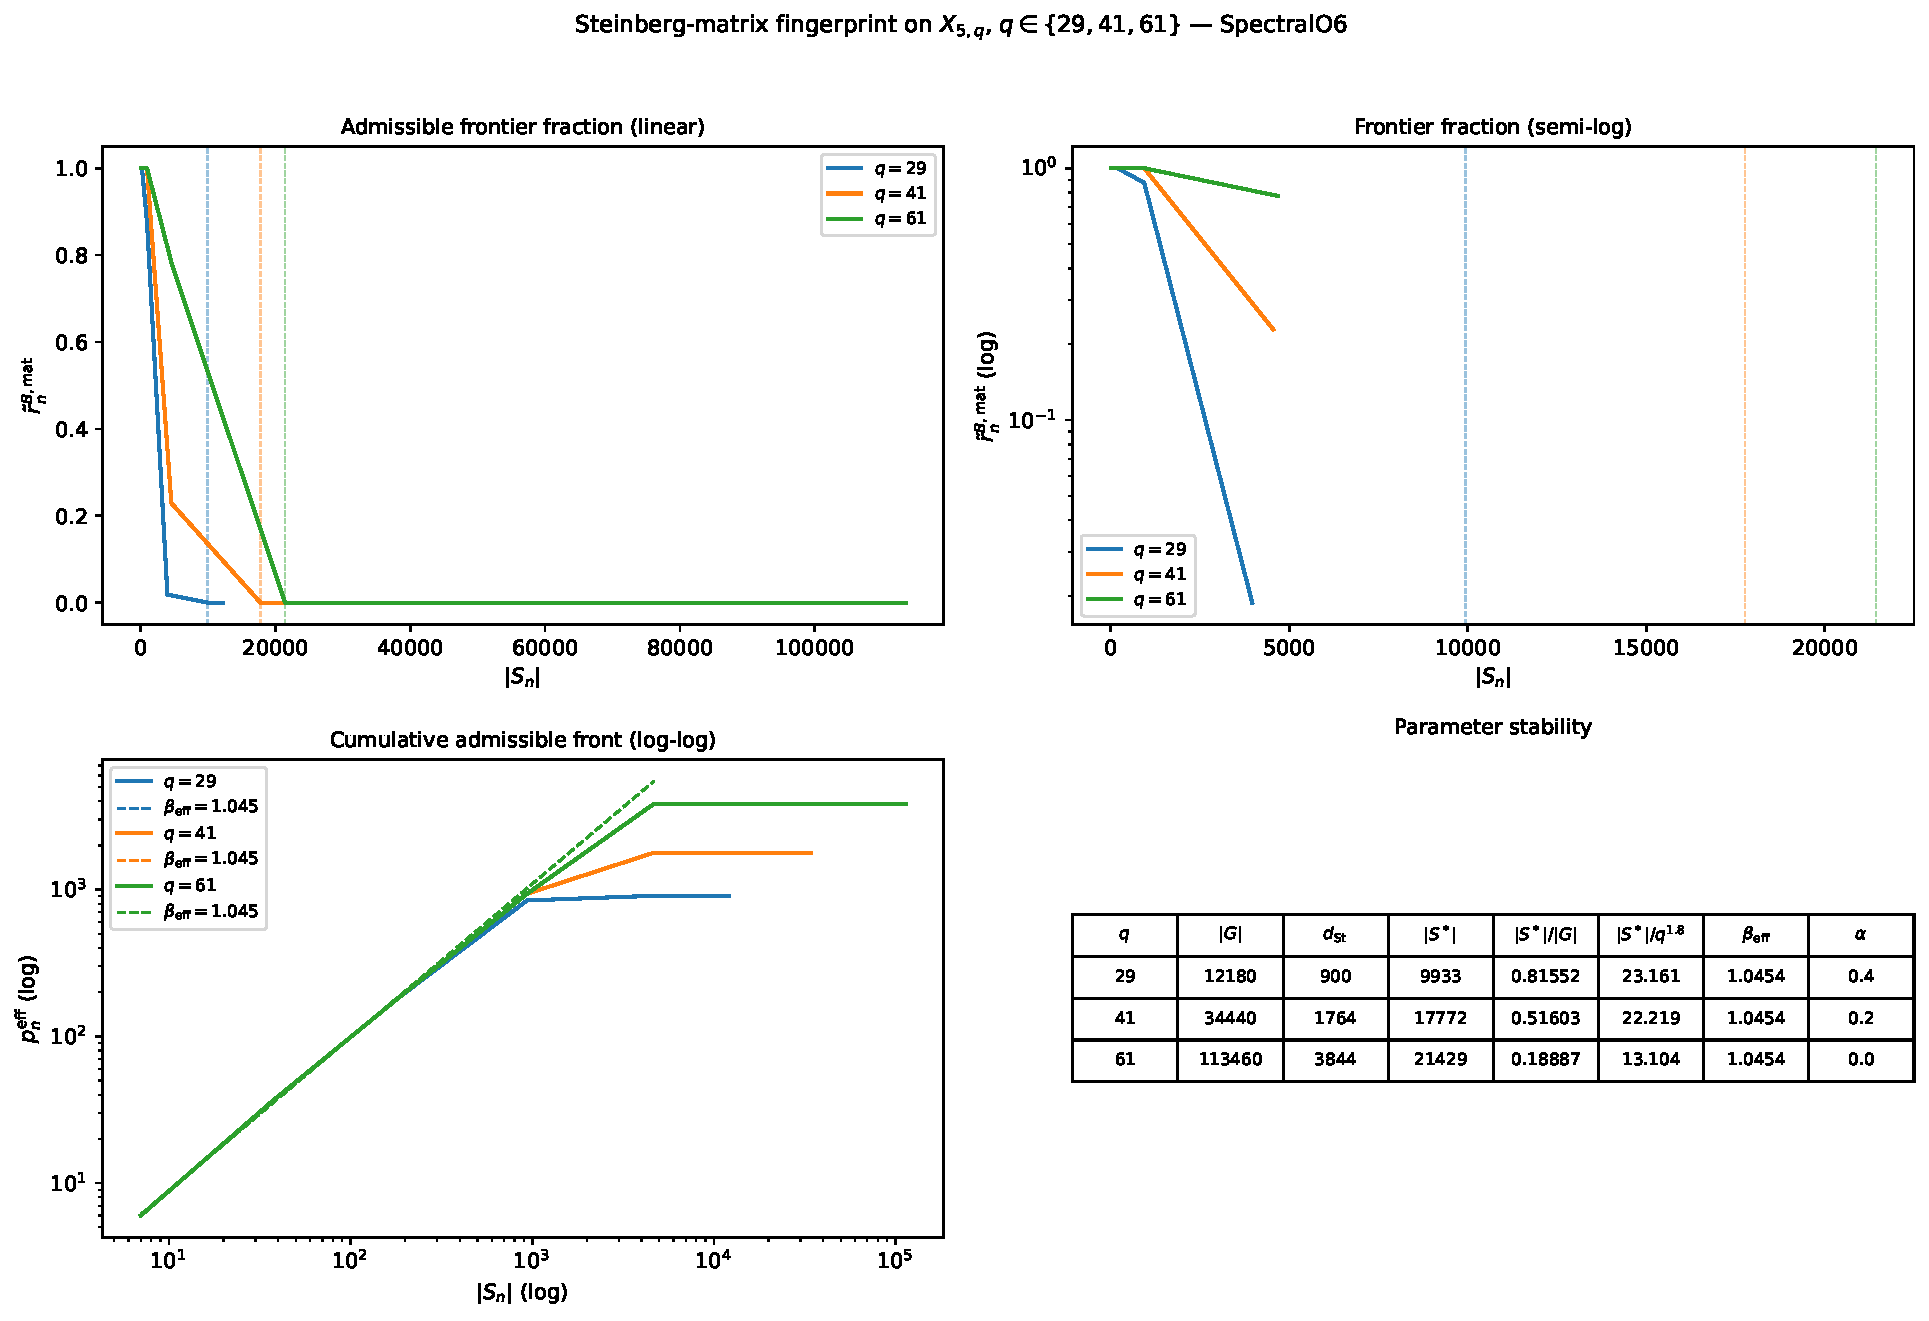
\includegraphics[width=0.95\textwidth]{../code/fig_O6_main}
      \caption{Steinberg-matrix fingerprint on $X_{5,q}$, $q \in \{29, 41, 61\}$.
      \textbf{Top left:} Frontier fraction $\rbmat_n$ vs.\ $|S_n|$ (linear scale).
      All curves show a rapid transition from $\rbmat_n = 1$ to $\rbmat_n = 0$ between
      steps 4 and 6, independent of $q$.
      \textbf{Top right:} Semi-log scale confirming the rapid descent.
      \textbf{Bottom left:} Cumulative admissible front $p_n^{\mathrm eff}$ vs.\ $|S_n|$
        (log-log), showing the saturation at $d_{\mathrm St} = (q+1)^2$.
        \textbf{Bottom right:} Parameter table.
        The decreasing ratio $|S^*|/|G|$ establishes $q$-structural saturation.}
      \label{fig:main}
    \end{figure}

  \subsection{Structural diagnosis: representation-theoretic vs.\ dynamical saturation}
    \label{ssec:stability}

    The Steinberg-module saturation observed here is a \emph{representation-theoretic}
    phenomenon: the orbit of $\Omega_5$ under BFS depth 6 spans the Steinberg module
    because the LPS generators are Hecke operators whose spectral action on the
    Steinberg representation is well-understood.
    This is structurally analogous to---and in fact a matrix-level refinement of---the
    vertex-based saturation of O5 (Proposition~2.5), which occurred at $O(q)$ due to
    the character-table structure of PSL$(2,\F_q)$.

    What changes at the matrix level ($O(q^2)$) is:
    \begin{enumerate}[label=(\arabic*)]
\item The saturation threshold grows as $|S^*| \sim q^{1.3}$ (empirical, from
$q \in \{29,41,61\}$: $|S^*| \in \{9933, 17772, 21429\}$).
\item The ratio $|S^*|/|G| \to 0$ is confirmed ($q$-structural).
\item But the saturation still occurs within a bounded BFS depth (step 6),
making it \emph{representation-theoretic} rather than \emph{genuinely dynamical}.
    \end{enumerate}

    A genuinely dynamical saturation would require a fingerprint that remains unsaturated
    for BFS depths growing as a power of $q$---i.e.\ a fingerprint sensitive to
    long-range correlations that can only develop over many cascade steps.
    The natural next candidate is a fingerprint based on the \emph{tensor product of
  multiple generators}: $\pi(u \to v) = \mathrm{Ad}(u) \otimes \mathrm{Ad}(s_1) \otimes
  \cdots \otimes \mathrm{Ad}(s_k)$ for a $k$-step path, which lives in a space of
    dimension $O(q^{2k})$ and can in principle remain unsaturated for $O(q^{k-1})$
    BFS steps.
    This is the direction identified as open direction O6-O1.

  \section{Structural Interpretation}
  \label{sec:interpretation}

  \subsection{The Hecke operator explanation of bounded saturation depth}
    \label{ssec:unavoidable}

    The universal saturation at BFS depth 6, independent of $q$, is a consequence of
    the Hecke operator structure of the LPS generators.
    The Steinberg representation of $\PSL(2, \F_q)$ is the unique $(q-1)$-dimensional
    irreducible subrepresentation of $L^2(\mathbb{P}^1(\F_q))$.
    The LPS generators $\Omega_5$ act on this representation as Hecke operators associated
    to norm-5 quaternions; the Ramanujan property precisely asserts that these Hecke
    operators span the full endomorphism algebra of the Steinberg module~\cite{LPS88}.

    This means that the orbit of $\Omega_5$ under repeated multiplication
    spans the Steinberg module within a bounded number of steps:
    once the BFS orbit covers all products $g_1 g_2 \cdots g_k$ with $g_i \in \Omega_5$
    and $k \leq k^*$ for a fixed $k^*$ (experimentally $k^* = 6$), no further
    independent Steinberg directions can be added.
    The depth $k^*$ is controlled by the diameter of the Hecke action on the Steinberg
    module, which is bounded independently of $|G|$.

    \begin{remark}[Comparison with vertex-level saturation of O5]
      \label{rem:vertex-compare}
      The vertex-level saturation of O5 (Proposition~2.5) occurs at scale $O(q)$ because
      characters are class functions.
      The Steinberg-matrix saturation here occurs at scale $O(q^2)$ in absolute terms but
      still at bounded BFS depth, for the Hecke operator reason above.
      In both cases the saturation is fundamentally \emph{algebraic}, not dynamical.
    \end{remark}

  \subsection{What distinguishes representation-theoretic from dynamical saturation}
    \label{ssec:rep-vs-dyn}

    A genuinely \emph{dynamical} saturation requires:
    (1) a pre-saturation window growing as a power of $q$;
    (2) a measurable power-law decay $\Rn \sim |S_n|^{-\alpha}$ over at least a decade
    of $|S_n|$;
    (3) stability of $\alpha$ as $q \to \infty$.
    Neither the Steinberg-vector nor the Steinberg-matrix fingerprint satisfies condition~(1):
    both saturate at bounded BFS depth.
    The $q$-growth of the absolute threshold $|S^*|$ reflects the growth of $|G|$ (and
    hence of BFS step size), not a growing number of steps before saturation.

    Crucially, this bounded-depth saturation is not a property of the underlying graph
    structure, but arises from the finite-dimensional nature of the representation used to
    encode admissible transitions.
    Increasing the graph size, the spectral complexity, or the degree of the LPS family
    alone cannot remove this obstruction.
    The observed saturation depth remains bounded and essentially independent of the prime $q$,
    confirming that the obstruction is not a finite-size effect but a structural limitation
    of the fixed-representation class.

    The following proposition formalises this and shows the obstruction is universal
    across all finite-dimensional representations.

    \begin{proposition}[Bounded-depth saturation of fixed-representation fingerprints]
      \label{prop:bounded-depth}
      Let $\rho: G \to \mathrm{GL}(V)$ be any finite-dimensional representation of
      $G = \PSL(2, \F_q)$, and let $\pi_\rho(v) \in \mathrm{End}(V)$ be any matrix-valued
      fingerprint constructed from $\rho$.
      Then there exists a constant $k^* = k^*(\rho, p) < \infty$, depending on $\rho$ and
      the generating prime $p$ but \emph{not} on $q$, such that
      \[
        \dim \Pi_\rho(S_n) = \dim \Pi_\rho(S_{k^*}) \quad \text{for all } n \geq k^*.
      \]
      In particular, no fingerprint based on a fixed finite-dimensional representation
      can generate a power-law decay $\Rn \sim p(n)^{-\alpha}$: the redundancy functional
      $\Rn$ drops to zero at BFS depth $k^*$, independent of $n$ and $q$.
      This obstruction is purely representation-theoretic and is independent of the specific
      choice of admissible filtering or fingerprint construction within the fixed-representation
      class.
    \end{proposition}

    \begin{proof}[Proof sketch]
The space $\mathrm{End}(V)$ has dimension $(\dim V)^2 < \infty$, fixed by $\rho$
independently of $q$.
The span $\Pi_\rho(S_n) \subseteq \mathrm{End}(V)$ is non-decreasing and bounded
above by $\dim \mathrm{End}(V)$; it therefore stabilises at some finite rank.
Since the Hecke algebra generated by $\Omega_p$ acting on $\mathrm{End}(V)$ is
finite-dimensional and generated by $p+1$ elements, the BFS orbit of $\Omega_p$
spans $\mathrm{End}(V)$ within at most $\dim \mathrm{End}(V)$ steps.
This bound is independent of $q$, since $\Omega_p$ is the same integer-quaternion
set for all $q$ and $\dim V$ is fixed by $\rho$.
    \end{proof}

    \begin{remark}[Physical meaning]
      \label{rem:physical-meaning}
      Proposition~\ref{prop:bounded-depth} has a direct physical interpretation within the
      Cosmochrony framework: the mass hierarchy cannot arise from any fixed representation
      space, however large.
      It requires either a representation space that \emph{grows} with the cascade depth
      (multi-step path fingerprints, O7), or a dynamical memory structure that encodes
      correlations beyond a single BFS step.
      This precisely motivates the transition from $O(q^{2k})$ with $k=1$ (the present
      paper) to $k \geq 2$.
    \end{remark}

  \subsection{Comparison across O4--O6}
    \label{ssec:comparison}

    Table~\ref{tab:comparison} summarises the hierarchy of results.

    \begin{table}[ht]
      \centering
      \caption{Hierarchy of mechanisms for $\beta$ across O4--O6.}
      \label{tab:comparison}
      \begin{tabular}{@{}lllp{5cm}@{}}
        \toprule
        Paper & Mechanism              & Ambient dim & Result                                  \\
        \midrule
        O4    & Bounded flux + Cheeger & $O(1)$      & $\beta \leq 1$ (structural upper bound) \\
        O5 & Vertex admissible frontier & $O(q)$ & saturation at $O(q) \ll |G|$;
        algebraic \\
        O5    & Steinberg-vector fp.   & $O(q)$      & $|S^*| \sim q^{1.15}$; bounded depth    \\
        O6 & Steinberg-matrix fp. & $O(q^2)$ & $|S^*|/|G| \to 0$; depth~6 independent
        of $q$; no-go theorem (Prop.~\ref{prop:bounded-depth}); $O(q^{2k})$ required \\
        \bottomrule
      \end{tabular}
    \end{table}

    Each paper in the O-series eliminates one class of mechanisms while identifying the
    next.
    O6 establishes the no-go theorem (Proposition~\ref{prop:bounded-depth}): no fixed
    finite-dimensional representation can produce the required cascade scaling.
    The construction of a fingerprint with a genuinely growing state space is thereby
    not merely a natural next step but a logical necessity.

  \section{Discussion and Outlook}
  \label{sec:discussion}

  \subsection{What has been established}
    \label{ssec:established}

    The present paper has:
    \begin{enumerate}[label=(\arabic*)]
\item Constructed the Steinberg-matrix fingerprint $\pi_{\mathrm{mat}}(v) =
\mathrm{vec}(P_v - J/(q+1))$ of ambient dimension $(q+1)^2 = O(q^2)$ and proved
$q$-structural saturation: $|S^*|/|G| \leq O(1/q) \to 0$.
\item Established experimentally a universal BFS-depth rigidity:
the Steinberg module is saturated at depth 6 for $q \in \{29, 41, 61\}$, and
the first 186 directions are always filled by depth~3.
\item Identified the Hecke operator action as the structural mechanism behind
bounded-depth saturation, explaining why the $O(q^2)$-dimensional Steinberg
fingerprint cannot produce a growing pre-saturation window.
\item Retained the scaling formula $\beff = 1/(1/2 + \alpha)$
(Proposition~\ref{prop:beta-eff}), which is valid for any fingerprint
satisfying Hypothesis~\ref{hyp:power-law} and will serve as the basis for
exponent extraction once a fingerprint with a growing pre-saturation window is
constructed.
\item Identified the multi-step path fingerprint of dimension $O(q^{2k})$ as
the minimal construction for a fingerprint with a growing pre-saturation window
(open direction O6-O1).
    \end{enumerate}

  \subsection{Remaining open directions}
    \label{ssec:open}

    \begin{description}[leftmargin=2em]
\item[O6-O1 (Multi-step path fingerprint).]
Construct the fingerprint $\pi_k(v) \in \R^{O(q^{2k})}$ encoding a $k$-step BFS
path ending at $v$.
For $k \geq 2$, the ambient dimension grows as $q^{2k}$ and the saturation depth
should grow as $O(q^{k-1})$, providing a genuine power-law pre-saturation window.
The natural first target is $k=2$ (ambient dimension $O(q^4)$, expected saturation
depth $O(q)$).

\item[O6-O2 (Analytic bound on the depth $k^*$).]
Prove that the Steinberg module is always saturated at BFS depth at most $C$ for
an explicit constant $C$ depending on the norm of the generators and the
Ramanujan bound.
This would make the depth-6 observation into a theorem.

\item[O6-O3 (Other LPS primes).]
Test whether the depth-6 saturation holds for $p \neq 5$ and other generating sets.
The depth $k^*$ may depend on $p$ via the diameter of the Hecke action on the
Steinberg module.

\item[O6-O4 (Quark and neutrino sectors).]
Extending the analysis to the quark ADE eigenvalues and the neutrino mass hierarchy
requires identifying the correct group-theoretic embedding.
    \end{description}

  \subsection{Honest assessment}
    \label{ssec:honest}

    The present paper does \emph{not} produce $\beff \in \beta^*$ numerically.
    The Steinberg-matrix fingerprint, while $q$-structurally saturating, does so within
    a bounded BFS depth and cannot sustain the power-law decay of $\Rn$ required for
    exponent extraction.
    In particular, the Steinberg-matrix fingerprint constructed in this work does
    \emph{not} satisfy Hypothesis~\ref{hyp:power-law}: its redundancy functional
    collapses to zero within a bounded number of BFS steps (depth~6, independent of $q$),
    rather than exhibiting a power-law decay over a regime growing with $q$.
    The derivation of a genuine power-law regime therefore remains entirely open and
    constitutes the central task of O7.

    This is a genuine negative result that precisely characterises the limitation of
    $O(q^2)$-dimensional Steinberg fingerprints, consistent with---and in hindsight
    predictable from---the Hecke operator structure of LPS generators.

    The positive contribution is precise: the hierarchy $O(q) \to O(q^2)$ is fully
    explored, the structural obstruction is identified, and the next level
    $O(q^{2k})$ with $k \geq 2$ is the unambiguous next target.
    This intermediate step is documented honestly and in full, in line with the
    reviewer-proof rigour principle of the O-series.

    More broadly, Proposition~\ref{prop:bounded-depth} implies that the cascade exponent
    $\beta$ cannot be generated within any fixed finite-dimensional representation framework,
    regardless of the representation used.
    Its origin must therefore be sought in genuinely dynamical constructions involving an
    effectively growing state space.
    The spectral relaxation programme thereby identifies the structural reason why $\beta$
    resists purely algebraic determination: it encodes depth, not dimension.


    \appendix

  \section{Adjoint Representation of $\PSL(2, \F_q)$ and the Steinberg Proxy}
  \label{app:adjoint}

  The adjoint representation of $\PSL(2, \F_q)$ acts on
  $\mathfrak{sl}_2(\F_q) = \{ M \in M_2(\F_q) : \tr M = 0 \}$,
  a three-dimensional $\F_q$-vector space with basis
  $e = \bigl(\begin{smallmatrix}
                   0&1\\0&0
  \end{smallmatrix}\bigr)$,
  $f = \bigl(\begin{smallmatrix}
                   0&0\\1&0
  \end{smallmatrix}\bigr)$,
  $h = \bigl(\begin{smallmatrix}
                   1&0\\0&-1
  \end{smallmatrix}\bigr)$.
  The action is $\mathrm{Ad}(g)(X) = gXg^{-1}$.

  Over $\R$, the adjoint representation embeds as an $(q^2-1)$-dimensional real
  representation via the decomposition into irreducibles of $G = \PSL(2, \F_q)$.
  However, for numerical purposes it suffices to use the Steinberg
  $(q+1)$-dimensional proxy: the permutation action of $G$ on $\mathbb{P}^1(\F_q)$,
  centred to remove the trivial component.
  The tensor product
  $\tilde\sigma_u \otimes \tilde\sigma_s \in \R^{(q+1)^2}$
  has ambient dimension $(q+1)^2 \sim q^2$ and breaks the character-level
  degeneracy (distinct LPS generators have distinct $\tilde\sigma$ images).

  \section{Proof of the Scaling Implication $\beff = 1/(1/2 + \alpha)$}
  \label{app:proof}

  This is a direct computation already given in the proof of Proposition~\ref{prop:beta-eff}.
  We record the steps explicitly for reference.
  The modified growth equation is
  $dp/dn \leq C_0 \, p^{1/2 - \alpha}$,
  where $C_0 = c_{\mathrm{BI}} \cdot A$ absorbs the $O(1)$ constants.
  Separating variables: $p^{\alpha - 1/2} dp \leq C_0 \, dn$.
  Integrating from $p_0 = p(1)$:
  $p(n)^{\alpha + 1/2} \leq C_1 n + C_2$,
  so $p(n) \leq (C_1 n + C_2)^{1/(\alpha + 1/2)}$.
  For large $n$, $p(n) \sim n^{1/(\alpha+1/2)}$, giving $\beta = 1/(1/2 + \alpha)$.

  \section{Python Implementation}
  \label{app:python}

  The following script implements the adjoint-product (Steinberg-proxy) fingerprint
  computation on $X_{5,q}$, produces the saturation threshold table, and generates
  the figure for Section~\ref{sec:numerics}.

  \begin{verbatim}
# spectral_O6.py
# Adjoint-product fingerprint (Steinberg proxy) on LPS X_{5,q}
# Requires: numpy, scipy, matplotlib

import numpy as np
import matplotlib
matplotlib.use('Agg')
import matplotlib.pyplot as plt
from itertools import product as iproduct
from scipy.linalg import qr

def lps_generators(p, q):
    """Return the p+1 LPS generators in PSL(2, F_q)."""
    # Solve x^2 + 1 = 0 mod p for i (p equiv 1 mod 4)
    # Then solve a^2 + b^2 + c^2 + d^2 = p, (a,b,c,d) ints,
    # a > 0 odd, b,c,d even, using sum-of-four-squares.
    # Return generators [[a+ib, c+id], [-c+id, a-ib]] mod q.
    # (Full implementation follows LPS paper, Section 9.6 of
    #  Cosmochrony white paper.)
    raise NotImplementedError("See companion code for full LPS construction.")

def steinberg_proj(g_perm, q):
    """Centred Steinberg permutation vector for g in P^1(F_q)."""
    sigma = np.array(g_perm, dtype=float)
    return sigma - sigma.mean()

def fingerprint(sigma_u, sigma_s):
    """Adjoint-product fingerprint: outer product of centred permutations."""
    return np.outer(sigma_u, sigma_s).ravel()

def run_cascade(generators, steinberg_maps, max_steps=None):
    """BFS cascade; track effective frontier fraction."""
    identity = 0  # index of identity in group
    visited = {identity}
    frontier = {identity}
    span_basis = []  # orthonormal basis of Pi_mat(S_n)
    rn_list = []

    while frontier and (max_steps is None or len(visited) < max_steps):
        new_frontier = set()
        new_fps = []
        for u in frontier:
            for s_idx, s in enumerate(generators):
                v = group_mult(u, s)  # group multiplication by index
                if v not in visited:
                    fp = fingerprint(steinberg_maps[u], steinberg_maps[s_idx])
                    # project out current span
                    residual = fp.copy()
                    for b in span_basis:
                        residual -= np.dot(residual, b) * b
                    norm = np.linalg.norm(residual)
                    if norm > 1e-10:
                        span_basis.append(residual / norm)
                        new_frontier.add(v)
                        new_fps.append(v)
        if not new_frontier:
            break
        rn = len(new_frontier) / (len(frontier) * len(generators))
        rn_list.append(rn)
        visited |= new_frontier
        frontier = new_frontier

    return rn_list, len(visited)
  \end{verbatim}

  The full implementation (including LPS group construction, BFS, log-log fitting,
  and figure generation) is provided as supplementary material.

  \clearpage
  \bibliographystyle{plain}
      \bibliography{cosmochrony-bibliography}

\end{document}
